\chapter{Exploring The Hopfield Model}
% This is where we describe our experiments. We insert plots, images, ....

We started out the analysis by experimenting with converge of patterns. We shall present two experiments, that provide some interesting insight for the reader into the Hopfield Model.

\section{Facial Recognition for Police criminal records}

This experiment describes how the Hopfield network might be used by a Police Office, in order to identify criminals. Since the police has a big database that contains facial images of criminals, the network can perform identify, given an image, which criminal is depicted.

Before being sent to the Hopfield model, the image suffers a few normalising transformations:
\begin{enumerate}
 \item the background is completely removed
 \item the image is scaled to 25x25 pixels.
 \item conversion first to grayscale, and then to only black or white pixels takes place
\end{enumerate}

In figure \ref{fig:criminal}, we present the convergence series for the input image of a criminal. The network used for this experiment had 400 neurons, running on images of 20x20 pixels. It clearly illustrates the how efficient the networks can be in these scenarios. However, the network might also convert to to spurious patterns, which might create problems in certain situations. See section \ref{spurious_patterns} for a more detailed description.

\begin{figure}[h]
  \centering
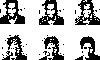
\includegraphics[scale=2]{images/convergence/all.png}
\caption{Convergence sequence for a criminal in the police database}
\label{fig:criminal}
\end{figure}

Furthermore, we have developed a GUI, powered by the underlying recognition core, to provide a friendly user experience, in addition to providing interactive facilities (figure \ref{fig:gui}). An overview of our the recognition system can be found in figure ~\ref{fig:system}.

\begin{figure}[h]
  \centering
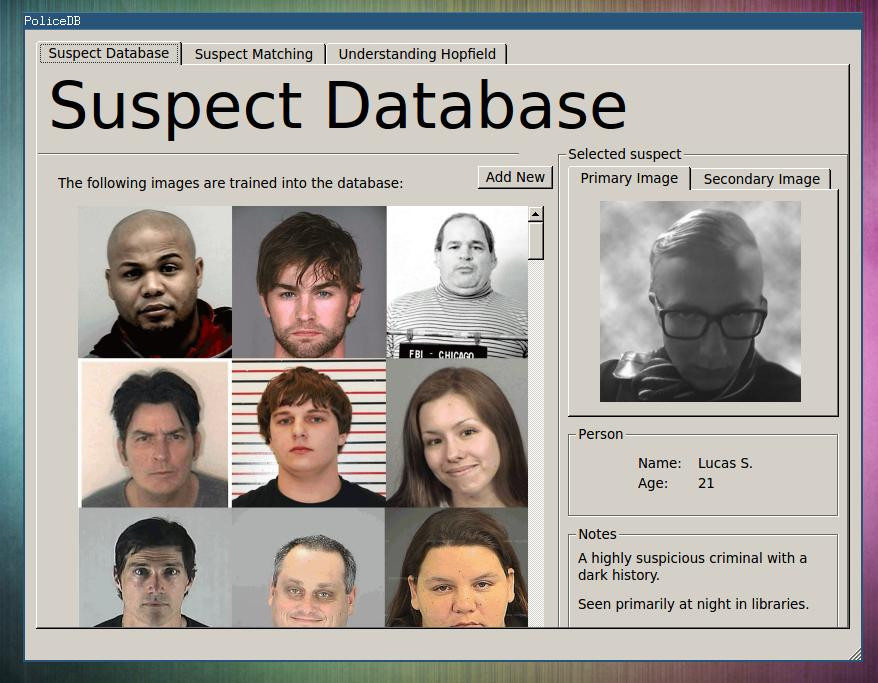
\includegraphics[scale=0.3]{screenshots-small/gui1.jpg}
\caption{GUI for a criminal record recognition system.}
\label{fig:gui}
\end{figure}

\begin{figure}[h]
  \centering
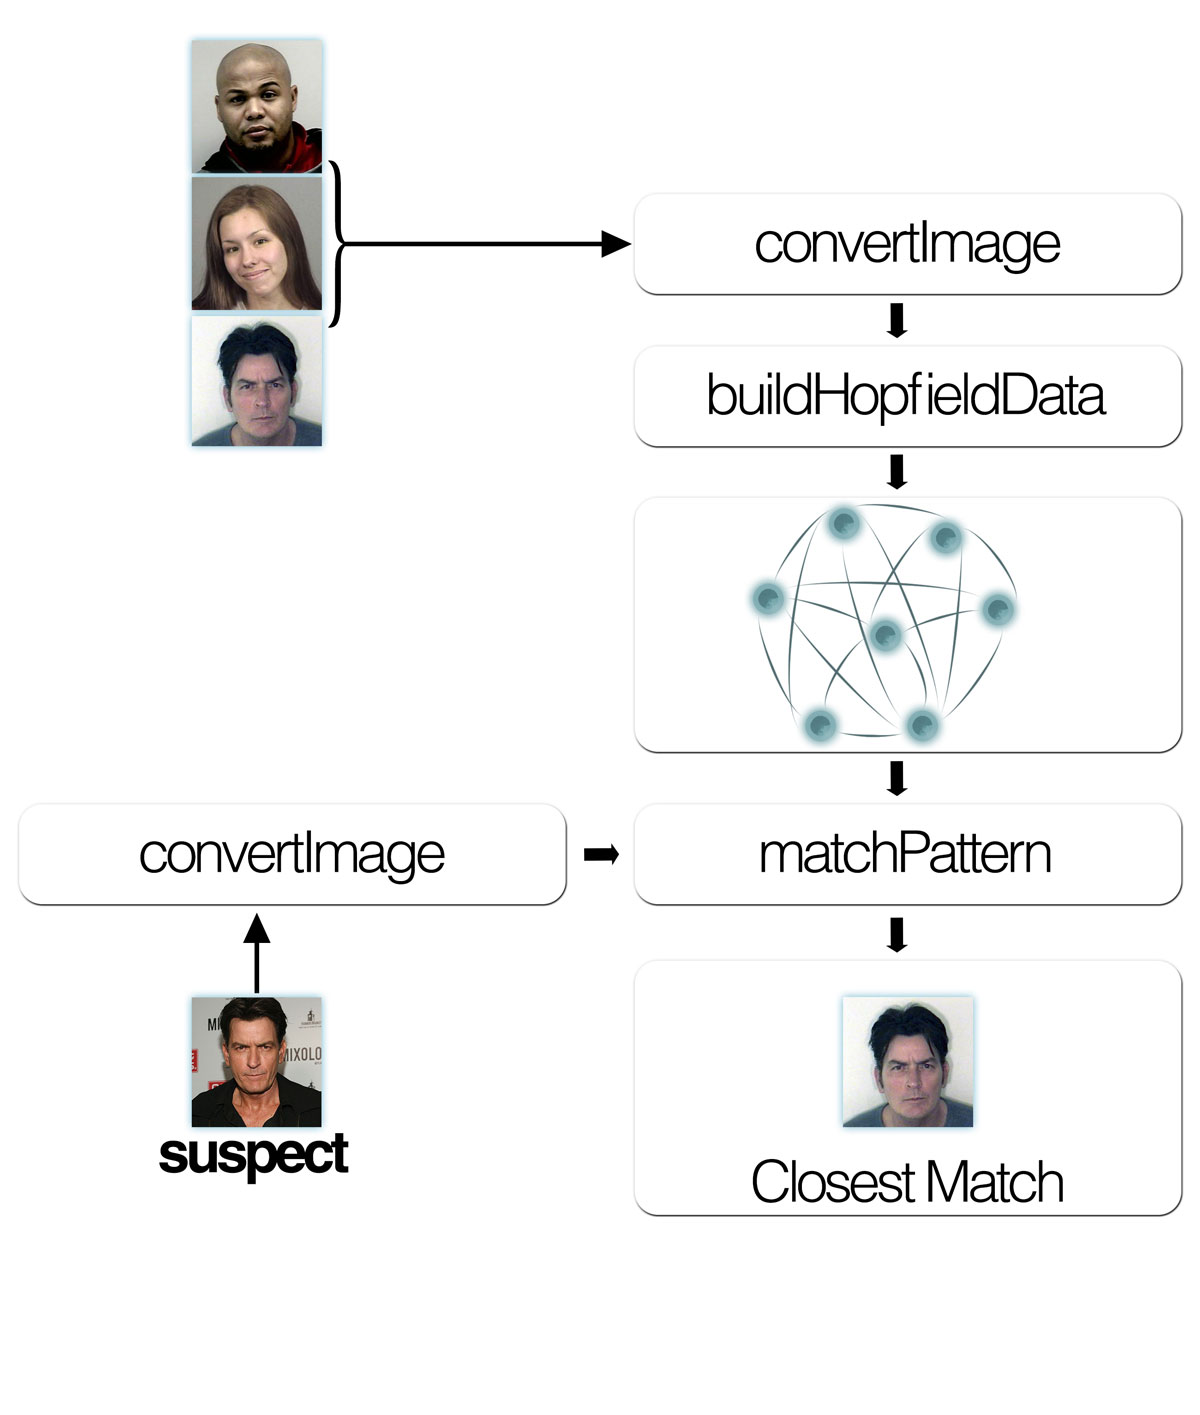
\includegraphics[scale=0.3]{recognition.jpg}
\caption{Outline of the Recognition System demonstrating how the various system components interact}
\label{fig:system}
\end{figure}


\section{Further analysis}

Our initial aim was to explore various properties of the attractors in a Hopfield Network. We are interested in studying, testing or challenging several ideas about the neural network:
\begin{itemize}
 \item Clusters of attractors: We are interested to see how the Hopfield network behaves when learning similarly correlated patterns. This implies training the network with a cluster of attractors, which will lower the capacity of the network. We believe that basin sizes will get smaller as the patterns get closer to each other.
 \item Super-Attractors: Find out what happens if the network is trained several times with the same pattern. We believe this super-attractor will have a larger basin size compared to the other attractors.
 \item Convergence: We plan to train the network with different types of attractors and find out to which ones patterns tend to converge.
\end{itemize}

\section{Basins of Attraction}
%I think we should move the measurements for the basins of attraction in here.
A basin of attraction for a particular attractor \(\alpha\) is defined as the set of all states that will eventually converge to \(\alpha\), under repeated update. Here, we are particularly interested in finding a way to measure the size of such a basin of attraction. A large basin size would provide stability for the attractor, since the states in the neighbourhood would converge to it. A small basin size for an attractor would mean that the network might never recall the pattern corresponding to that attractor.

\subsection{Measuring the Basin Size using the Storkey-Valabregue technique}
\label{storkey_basin_size}

 A large part of our experiments were thus dedicated to measuring basin sizes of different attractors, clusters of attractors and a newly introduced concept of \emph{Super-Attractors}, in section ~\ref{super_attractors}.

 A recognised scientific method for calculating the basin size is the Storkey-Valabregue measurement. This can be computed as follows:

 \begin{enumerate}
  \item Initially n = 1
  \item Choose an initial fixed point corresponding to a stored pattern \(\mu\)
  \item \label{itm:choose radius} Choose some initial normalised Hamming radius \(r=r_{0}\)
  \item Let the set A be all the states Hamming-distant \( nr \) from the fixed point
  \item Sample 100 states from A
  \item Calculate how many of these states are attracted to the fixed point. Denote this number \( t_{\mu}(r) \)
  \item If \( t_{\mu}(r) \) is smaller than 90, stop and return \(nr\)
  \item Increment \(n\) by a suitable amount and repeat from (\ref{itm:choose radius})
  \item Repeat for each attractor.
 \end{enumerate}

% TODO: This algorithm is implemented in the Haskell function ...


\section{Generating Clusters of Attractors}

There are various ways of generating clusters of attractors (i.e. attractors that have a low Hamming distance between each other). We shall present two different methodologies that can be used to generate them.

One way is to start with a root pattern and then reverse each bit with a probability p. The new patterns can be interpreted as noisy versions of the root pattern. We shall denote this procedure T1.

\subsection{Generating Gaussian-Distributed Clusters}

Another objective of this work was to analyse patterns that are extracted according to a Gaussian distribution with a specific mean and variance.

Since the state space is \( 2^N \) for a network of N neurons, the Gaussian Distribution will have to be defined over a huge set of states. This is highly non-trivial, since we are dealing with binary patterns, that cannot be ordered in an easy way.

In this case, we will use Mancinelli's method for sampling Gaussian distributed patterns \cite[p.~33]{federico}. We tackle this issue using the simplest possible approach: to draw numbers from a Normal Distribution and then translate them into patterns that will preserve the distance between them. Formally, if \(x\) and \(y\) were drawn and \( |x-y|=\delta\), then the Hamming distance between the encoded patterns \(x'\) and \(y'\) would also be \( d(x',y')=\delta\).

\subsubsection{Encoding of the patterns}

In order to encode a number into a binary pattern, we first round the number to the nearest integer. Let k be the integer obtained as such. Now, from left to right, we set to 1 all the bits in locations 1..k of our pattern. The remaining bits are set to -1.

For example, if the pattern size is 7 and the integer obtained is 4, we get the following pattern: [1,1,1,1,-1,-1,-1].

\subsubsection{Limitations of the encoding}

Although the method has a big advantage for simplicity, we can only obtain N different patterns out of all \( 2^N\) patterns available in the state space. However, we can regain capacity if we start flipping bits, while at the same time keeping constant the hamming distance to some certain mean pattern \(\mu\).

Another idea would be to extend our distribution to a multi-variate distribution. In this case, the capacity of the network would increase from \(N\) to \(\frac{n}{k}^k\), where k is the number of dimensions.

Unfortunately, we did not have enough time to implement these ideas, so we only experimented with the naive encoding of patterns described above.


\section{First experiments with basin sizes}
\label{sec:fexp}

In this section we shall introduce the experiments that we used to analyse various properties of the Hopfield Network. We remind the reader about the two methods that we are going to use for generating clusters of attractors:
\begin{itemize}
 \item T1: We start with a root pattern \(\mu\), and generate patterns by flipping each bit from \(\mu\) with probability \(p\).
 \item T2: This method is generating Gaussian-distributed patterns. We sample several numbers from a normal distribution with a certain mean and variance, and then encode each number into patterns of the form [1,1,1,-1,-1].
\end{itemize}


\subsection{Basin Size for One Cluster using T1}

Our first experiment is showing us the basin sizes for increasing values of p, the probability of flipping a bit. Method T1 is used, for a Hopfield Network of N neurons.

\begin{easylist}[enumerate]
\ListProperties(Style2*=,Numbers=a,Numbers1=R,FinalMark=.)
& We generate a random pattern \(\mu\)

& For all values of probability p from 0 to 0.5

    && Starting from \(\mu\) we generate P patterns using T1, and give them to the Hopfield network in order to be learned according to Hebb or Storkey rule.

    && We measure the basin size for all the patterns learned using the Storkey-Valabregue measurement and take their mean.
\end{easylist}

\begin{figure}[h]
  \centering
  \begin{tikzpicture}
\begin{axis}[
xmin = 0,
ymin = 0,
xlabel = $p$-value,
ylabel = Average Basin Size
]

\addplot [
color = black,
mark = *, % A filled circle
only marks,
smooth  % draw smooth curve
] table [
y = mean
] {data-T1-onecluster-100.csv};

\end{axis}
\end{tikzpicture}

\caption{Average Basin size of patterns belonging to one cluster generated using T1}
\label{fig:plot-T1-onecluster}
\end{figure}

\subsubsection{Comments}

The results are displayed in figure \ref{fig:plot-T1-onecluster}. This initial experiment is confirming not only what Mancinelli obtained \cite{federico}, but also what we already know from theory: A Hopfield network that is trained with similar patterns loses capacity. Although we are not measuring capacity here, the basin size is strongly correlated to that.

Initially, when p is zero, we observe a huge value of 24 for the basin size. This is easily explained, since all the patterns generated are the the same as the root pattern. Subsequently, the network is trained with the same patterns that have the effect of creating a super-attractor with a huge basin size.

When p is between 0 and a critical value of 0.35, the basin size is 0, since the patterns are too close to each other and don't have enough space to fit basins of attraction between them. As soon as p goes over 0.35, the basins start to increase until a maximum size of 11.

\subsubsection{Further explanation of the results}

The results can also be easily understood and visualised in figure \ref{fig:basins}. For small p values, the attractors formed in the network are too close to each other to allow room for any basins of attraction (apart from the attractors lying at the edge of the cluster). When the p-value is high, the attractors become more disperse, leaving room for larger basins. It is also worth mentioning that the basin shapes are not necessarily hyper-spherical.


\begin{figure}[h]
  \centering
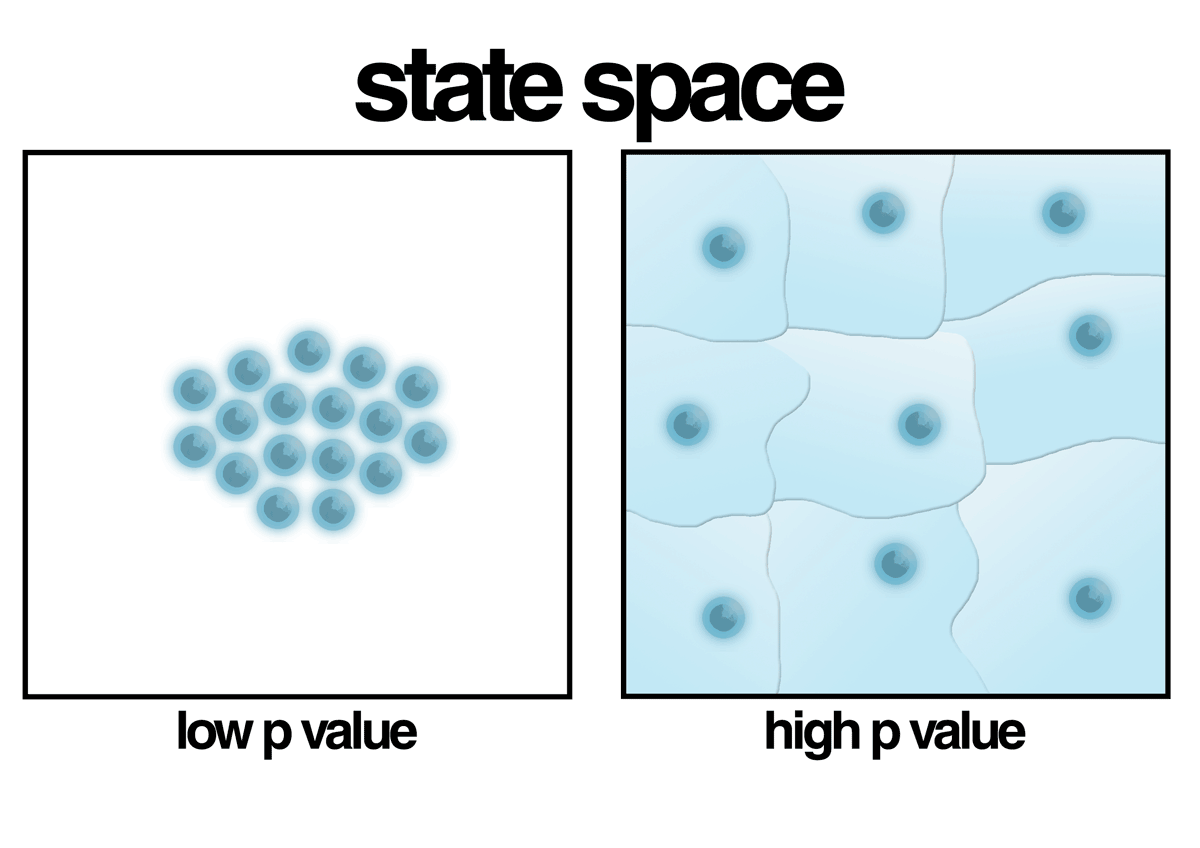
\includegraphics[scale=0.25]{images/basins_of_attraction.png}
\caption{Illustration of clusters of attractors generated using T1, with different p-values. }
\label{fig:basins}
\end{figure}


\subsection{Basin Size for Two Clusters using T1}

This experiment is similar to the previous one, however it contains two clusters this time. The value \(p_{1}\) for one cluster will stay the same (fixed at 0.45), while \( p_{2}\), corresponding to the second cluster, will vary in the range [0-0.5]. Method T1 is used, for a Hopfield Network of N neurons. The procedure is given below:
\newline
\begin{easylist}[enumerate]
\ListProperties(Style2*=,Numbers=a,Numbers1=R,FinalMark=.)
& We generate 2 random patterns \(\mu_{1}\) and \(\mu_{2}\), corresponding to clusters \( C_{1} \) and \( C_{2} \).

& We generate P patterns for \( C_{1} \), using T1 with associated probability \( p_{1}=0.45\).

& For all values of probability \( p_{2} \) from 0 to 0.5

    && Starting from \(\mu_{2}\) we generate P patterns using T1 with associated probability \( p_{2} \), and give them to the Hopfield network in order to be learned according to Hebb or Storkey rule.

    && For both sets of patterns, we measure the mean basin size using the Storkey-Valabregue measurement and plot the values on the graph.
\end{easylist}

We will be interested to observe how can the probability p influences the basin sizes. For this reason, we have run two experiments, in which we are outputting the basin sizes for cluster 1, in which p varies. The

\subsubsection{Comments}

\begin{figure}[h]
  \centering
  \begin{tikzpicture}
\begin{axis}[
xmin = 0,
xmax = 0.5,
ymin = 0,
xlabel = p-value of cluster 2,
ylabel = Average Basin Size,
width=12cm,
height=9cm
% legend
% legend style={at={(1,0.5)},anchor=east}
]

\addlegendentry{Cluster 1 with $p$ = 0.2} ;

\addplot [
color = red,
mark = x, % A filled circle
% mark = none,
only marks,
smooth  % draw smooth curve
] table [
y = mean-new
] {data-T1-twocluster-100-0.4.csv};

\addlegendentry{Cluster 1 with $p$ = 0.4} ;


\addplot [
color = blue,
mark = triangle, % A filled circle
only marks,
smooth  % draw smooth curve
] table [
y = mean-new
] {data-T1-twocluster-100-0.2.csv};

\addlegendentry{Cluster 1 with $p$ = 0.2} ;



\end{axis}
\end{tikzpicture}

\caption{Average Basin size of patterns belonging to Cluster 2, generated using T1}
\label{fig:plot-T1-twocluster}
\end{figure}

This latter experiment seems to suggest that the probability $p$ of flipping bits in the pattern doesn't actually influence the basin sizes of attractors in Cluster 1. The same behaviour has been observed in the previous graph, and this is the case especially when the root images, that are randomly generated, are far away from each other.




\subsubsection{Link to attachment theory}
A network having been trained with two clusters of patterns can be interpreted, in attachment theory, with an infant that has been exposed to two different caregivers. The patterns can be for example, visual or auditory memories describing the 2 caregivers.



\section{Experiments with Gaussian-distributed patterns}

In this section we are testing clusters of patterns that have been generated using a normal distribution. We are expecting to get similar results to the T1 method, since by the Central Limit Theorem, the Binomial distribution ~ B(N, p) is nicely approximated by a Gaussian distribution with mean N(Np, Np(1-p)). Since in the previous experiments, we used to increase the probability p of flipping a bit, this now translates to increasing the standard deviation of the normal distribution.


\subsubsection{Comments}

\begin{figure}[h]
  \centering
  \begin{tikzpicture}
\begin{axis}[
xmin = 0,
ymin = 0,
xlabel = Standard deviation,
ylabel = Average Basin Size
]

\addplot [
color = black,
mark = *, % A filled circle
only marks,
smooth  % draw smooth curve
] table [
y = mean
] {data-T2-onecluster-100.csv};

\end{axis}
\end{tikzpicture}

\caption{Average basin sizes of one cluster generated using T2}
\label{fig:plot-T2-onecluster}
\end{figure}

The results here are quite surprising. The experiment with Gaussian-distributed patterns shows us that the basin sizes decrease exponentially as standard deviation increases. This might be the case because at low standard deviation, the patterns would repeat themselves and create small super-attractors that have big basin sizes.
This is in contradiction with what we obtained previously, when using method T1, and further details and possible explanations are given in section \ref{inconsistencies}.

\subsection{Basin Size for Two Clusters using T2}

\subsubsection{Comments}

\begin{figure}[h]
  \centering
  \begin{tikzpicture}
\begin{axis}[
xmin = 0,
ymin = 0,
xlabel = Standard Deviation of Cluster 2,
ylabel = Average Basin Size of Cluster 2,
width=12cm,
height=9cm
% legend
% legend style={at={(1,0.5)},anchor=east}
]

\addplot [
color = red,
mark = x, % A filled circle
% mark = none,
only marks,
smooth  % draw smooth curve
] table [
y = mean-new
] {data-T2-twocluster-100-5.csv};

\addlegendentry{Cluster 1 with $\sigma$ = 5.0} ;


\addplot [
color = blue,
mark = triangle, % A filled circle
only marks,
smooth  % draw smooth curve
] table [
y = mean-new
] {data-T2-twocluster-100-10.csv};

\addlegendentry{Cluster 1 with $\sigma$ = 10.0} ;


% \addplot [
% color = orange,
% mark = o, % A filled circle
% only marks,
% smooth  % draw smooth curve
% ] table [
% y = mean-avg
% ] {data-T2-twocluster-100.csv};

% \addlegendentry{Aggregate} ;


\end{axis}
\end{tikzpicture}

\caption{Average basin size for two clusters generated using T2}
\label{fig:plot-T2-twocluster}
\end{figure}

This experiment has been run on a network of 100 nodes, with 2 clusters of patterns:C1, with fixed standard deviation $\sigma_{1}$, and C2, with varying standard deviation $\sigma_{2}$. We have run two different trials, with $\sigma_{1}$ = 5 or 10.

As it can be easily noticed in the graph, the standard deviation does not have any effect on the basin size of the clusters. This seems to suggest that a more disperse cluster will not be affected by neighbouring attractors.


\section{Super Attractors}
\label{super_attractors}
In the context of learning models such as the Hopfield model, we define a super attractor as an attractor resulting from training a model with multiple occurrences or instances of some stored pattern. The degree of a super attractor denotes the number of occurrences of its corresponding pattern in the training set.


In the context of modelling Attachment theory, a super attractor may represent repeated interactions with the primary care giver. Clearly, it is of interest to investigate the properties of such an attractor; in particular establishing the existence and, if existent, the type of relationship between the degree of the super attractor and the extent of its dominance, or stability, over the space of patterns.


\subsection{Single super attractor}

% Define variables
\newcommand{\psuper}{$p_{super}$}
\newcommand{\prandom}{$\overrightarrow{p}_{random}$}

\begin{enumerate}


\item Fix N, the number of neurons.

\item \label{itm:choose pattern} Choose a random pattern \psuper, which signifies the primary care giver.

\item Choose a number of random patterns \prandom, such that the Hamming distance between \psuper and each of \prandom is between 25\% and 75\%.

The range forms a ball centred at 50\% Hamming distance\footnote{The percentage Hamming distance is simply the Hamming distance divided by the number of bits N} with an arbitrary radius, chosen such that the probability of a \prandom falling into \psuper's basin of attraction is small. This is done to avoid forming clusters of attractors, which we deal with separately in Recall that the Hopfield network is sign blind, and as a result the inverse of \psuper, $p_{super}^{-1}$, forms a symmetric super attractor. It is for this reason that a symmetric range about 50\% is chosen.

\item Choose a degree $d$ for \psuper and train a Hopfield network using $\overrightarrow{p}^d_{super}$ ($d$ instances of \psuper) and \prandom.

\item Measure the basin of attraction of \psuper using the Storkey-Valabregue method.

\item Repeat from (\ref{itm:choose pattern}) for various values of degree $d$.

\end{enumerate}


In our experiment 100 neurons are used, and the network is trained with 16 random patterns in addition to the super attractor. It is run with degree values {[}1, 2, 4, 8, 16, 32{]}. The entire procedure is repeated 800 times for various randomly chosen \psuper and \prandom. The average results obtained are summarised in ~\ref{fig:one super plot}.

This experiment can be replicated by running \texttt{Experiment.hs}.

\begin{figure}[h]
  \centering
\begin{tikzpicture}
\begin{axis}[
xmin = 0,
ymin = 0,
xlabel = Degree,
ylabel = Average Basin Size
]

\addplot [
color = black,
mark = *, % A filled circle
only marks,
smooth  % draw smooth curve
] table [
y = mean
] {data-one-super.csv};

\end{axis}
\end{tikzpicture}

\caption{Average basin of attraction for a super attractor with varying degrees.}
\label{fig:one super plot}
\end{figure}


The results show that as the super attractor's degree is increased, its basin of attraction also increases. Also note that this increase appears to approach the singularity at 50\% Hamming distance, which is consistent with our knowledge of \psuper's symmetrical counterpart. The very fast initial growth also indicates that super attractors in general very stable and demonstrate strong dominance over the space of patterns.


Linking back to the Attachment theory model, this may be interpreted as depicting the strong influence of repeated and consistent interaction with the child, represented by a super attractor of increasing degree. In particular, it exhibits its dominance over distantly scattered, unrelated influences, which are represented by the random patterns.



\subsection{Two super attractors}


% Define variables
\newcommand{\poriginsuper}{$p_{origin}$}
\newcommand{\pnewsuper}{$p_{new}$}
\newcommand{\dorigin}{$d_{origin}$}
\newcommand{\dnew}{$d_{new}$}

\begin{enumerate}

\item Fix N, the number of neurons.

\item Fix a degree \dorigin, for all chosen \poriginsuper from (\ref{itm:choose two super}).

\item \label{itm:choose two super} Choose a random pattern \poriginsuper, which signifies the primary care giver.

\item Choose a random pattern \pnewsuper, such that the Hamming distance between \poriginsuper and each of \pnewsuper is between 25\% and 75\%. This could symbolise the training due to either an alternate and influential care giver, or that resulting from a retraining period.


\item Choose a number of random patterns \prandom, such that the Hamming distance between \poriginsuper and each of \prandom is between 25\% and 75\%.

Note that while this allows for the possibility of forming a cluster in the vicinity of \pnewsuper, in practice the probability of this occurring is negligible.


\item Choose a degree \dnew for \pnewsuper and train a Hopfield network using \prandom, \dorigin instances of \poriginsuper, and \dnew instances of \pnewsuper

\item Measure the basins of attraction for each of \poriginsuper and \pnewsuper using the Storkey-Valabregue method.

\item Repeat from (\ref{itm:choose two super}) for different value of degree \dnew.

\end{enumerate}

In our experiment 100 neurons are used, and the network was trained with 8 random patterns in addition to the original and new super attractors, \poriginsuper and \pnewsuper, respectively. \poriginsuper is given a fixed degree, \dorigin, of 8. This value was chosen as being the smallest point of stability from the previous experiment ~\ref{fig:one super plot}, beyond which increasing the degree further does not greatly impact the basin of attraction. It is run with \dnew degree values {[}1, 2, 4, 8, 16, 32{]}. The entire procedure is repeated 634 times for various randomly chosen \poriginsuper, \pnewsuper and \prandom. The average results obtained are summarised in ~\ref{fig:two super plot}.

This experiment can be replicated by running \texttt{ExperimentSuper2.hs}.

\begin{figure}[h]
  \centering
\begin{tikzpicture}
\begin{axis}[
xmin = 0,
ymin = 0,
xlabel = Degree,
ylabel = Average Basin Size
]

\addplot [
color = red,
mark = *, % A filled circle
only marks,
smooth  % draw smooth curve
] table [
y = mean-origin
] {data-two-super.csv};


\addplot [
color = blue,
mark = *, % A filled circle
only marks,
smooth  % draw smooth curve
] table [
y = mean-new
] {data-two-super.csv};

\end{axis}
\end{tikzpicture}

\caption{Average basin of attraction for the two super attractors, \poriginsuper having a fixed degree, \dorigin, of 8, and varying the degree, \dnew, of \pnewsuper.}
\label{fig:two super plot}
\end{figure}


The results clearly reveal that increasing the degree of the new pattern increases its own basin of attraction, and decreases that of the original pattern. This relationship is symmetrical, as can be observed by the shape of the graph, in addition to the intersection point, which occurs (roughly) near the point (8 , 8) where both patterns have the same degree of 8. By random choice of original pattern, and random choice of new pattern (subject to a Hamming distance of 25\% to 75\% from the original pattern), we can claim that the basin of attraction depends solely on the relative degrees of the two patterns, and is independent of the actual patterns themselves. This is also consistent with the symmetry observed.

This also fits in nicely nicely with in the Attachment theory interpretation. The original pattern as before represents the consistent interactions with a primary care giver. The new pattern may represent the consistent, yet significantly different, interactions with an alternate and influential care giver, perhaps the other parent of the child or a relative with whom they have developed a close relationship. Intuitively, the care giver which has more interactions would exert a stronger influence, undermining the dominance of the other care giver, and indeed the impact of any other interactions.

In relation to retraining, the new pattern may also be taken to represent the influences arising due to the undertaken retraining phase. We find that, similar to the above, increasing the number of interactions due to retraining further ingrains its dominance, and dilutes that of the previous interactions due to the primary care giver or otherwise.


% undefined variables
\let\psuper\undefined
\let\poriginsuper\undefined
\let\pnewsuper\undefined
\let\dorigin\undefined
\let\dnew\undefined
\let\prandom\undefined





